% Chapter 4: Hardware/Software Implementation and Testing

\chapter{Hardware/Software Implementation and Testing}
\label{ch:impl}

This chapter describes how the autonomous UGV system was implemented and tested. The development was carried out in two main components: the UGV platform and onboard software stack, followed by the communication infrastructure and ground control station with the AI perception pipeline. The chapter also covers the operator user interface, the scope of evaluation, unit testing, and function testing with explicit requirements.

\section{Development Stages}

\subsection{Component 1: UGV Platform and Onboard Stack}

The first component encompasses the physical robot and all software that runs on the Raspberry Pi~4 onboard the UGV. Implementation followed the architecture described in Chapter~\ref{ch:method}, with the following as-built choices.

\textbf{Hardware implementation.} The UGV chassis is a differential-drive or skid-steer base capable of carrying the compute unit, sensors, battery, and up to two deployable mesh nodes. The main computer is a Raspberry Pi~4 with 8\,GB RAM, running Ubuntu 22.04 LTS \cite{ubuntuhelp} and ROS~2 Humble \cite{ros2humble}. It was selected for cost, availability, and sufficient performance for real-time Cartographer \cite{hess2016} at 10\,Hz. Velocity commands from the navigation stack are published to the standard \texttt{cmd\_vel} topic and converted to motor outputs by a low-level controller.

Sensing is provided by a YDLidar X3 2D LiDAR \cite{ydlidar} (12\,m range, approximately 1° resolution, 10\,Hz) connected via USB--UART, which supplies scan data for SLAM. A Microsoft Kinect v1 is used as an RGB-D camera under budget constraints; its point cloud is fused into the Nav2 \cite{nav2dwb} local costmap to improve obstacle avoidance for overhangs and table legs that the 2D LiDAR cannot see. Vision for the operator is provided by a USB webcam (main camera) and an ESP32-CAM (rear), both at 720p and 15\,fps. The platform is equipped with headlights and a strobe mode for low-light operation and to attract attention. A TP-Link Archer C6 router on the UGV serves as the main Wi-Fi access point, with the Pi connected via Ethernet. Deployable mesh nodes are built around ESP32 DevKit modules running ESP-WiFi-MESH \cite{espmesh}; each node is powered by a 2500\,mAh LiPo and is deployed by a servo mechanism along the UGV's path. Upon deployment, each node is added to the routing table so that the mesh self-heals and extends coverage. A LoRa SX1278 radio provides last-resort telemetry and return-to-base commands. The UGV is powered by a 24\,V pack made from two 3s3p 18650 cell groups in series, yielding almost two hours of continuous operation at a cruise speed of 0.2\,m/s. A summary bill of materials is given in Appendix~\ref{app:components}.

% --- FIGURE: System architecture ---
\begin{figure}[htbp]
\centering
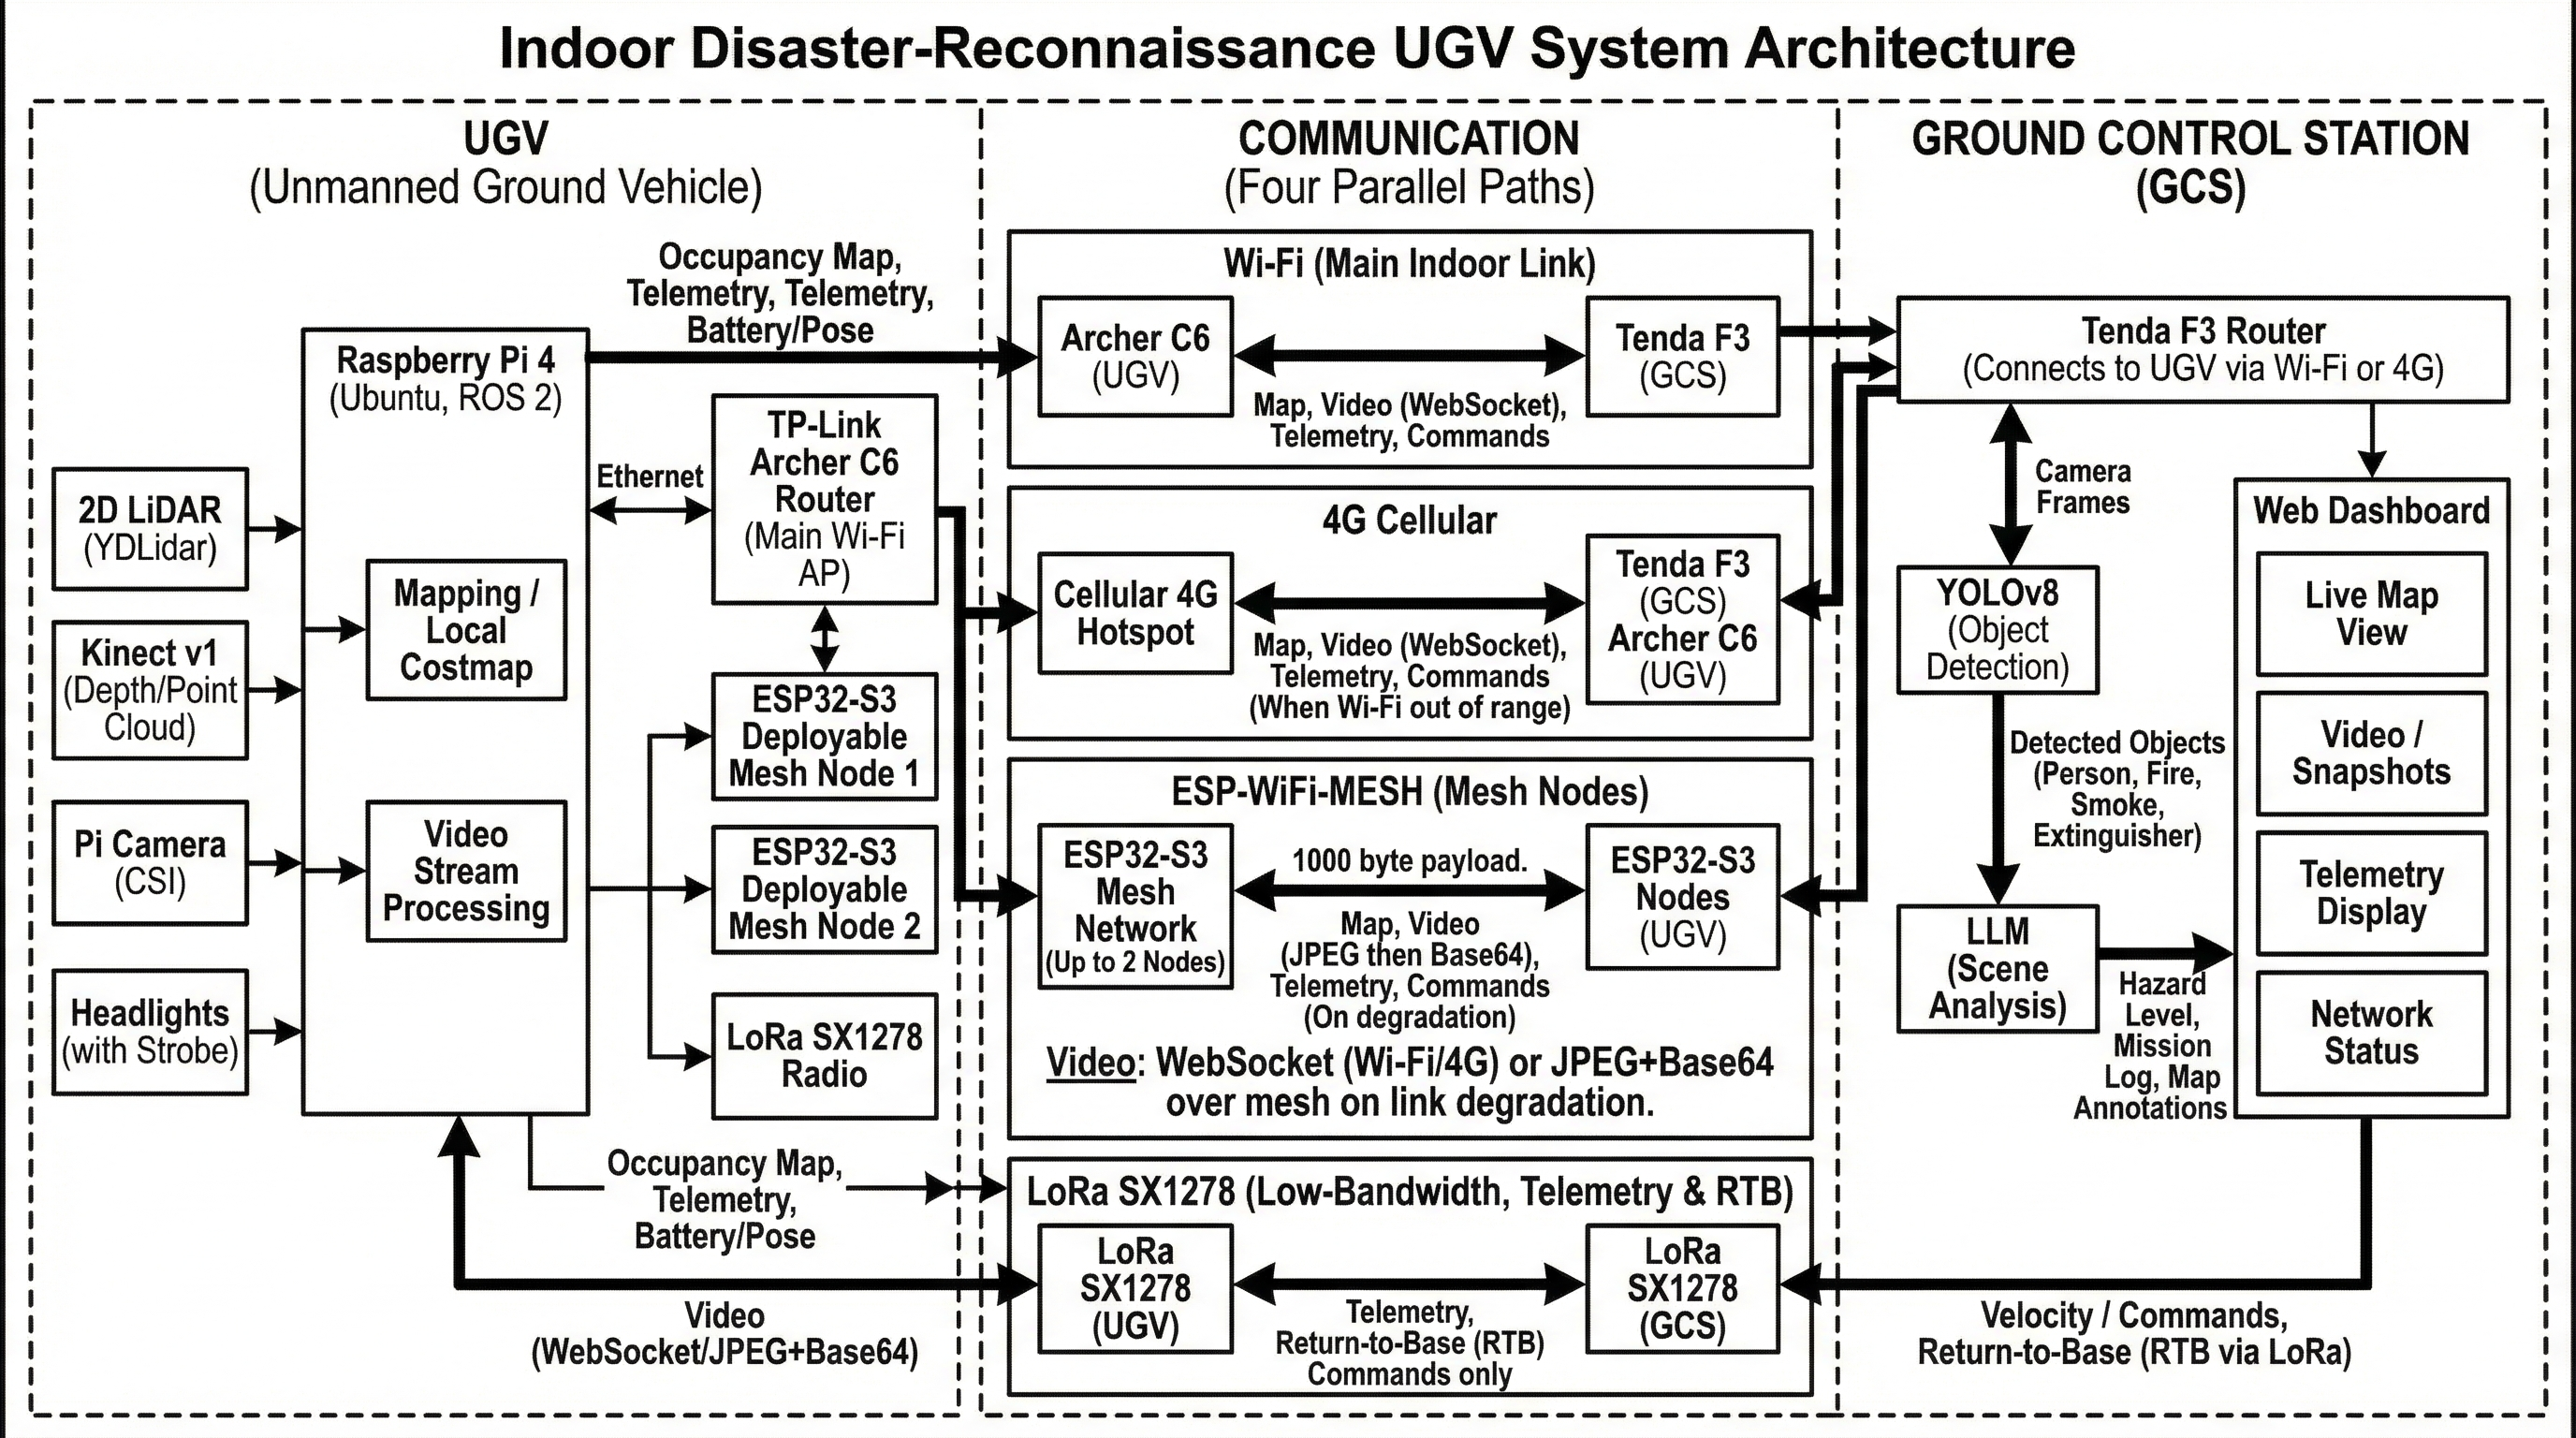
\includegraphics[width=0.85\textwidth]{figures/system_architecture.jpg}
\caption{System architecture: UGV, multi-tier network, and GCS.}
\label{fig:arch}
\end{figure}

Figure~\ref{fig:ugv_views} shows the as-built platform from the front, side, and rear.
\begin{figure}[htbp]
\centering
\begin{minipage}[t]{0.32\textwidth}
\centering
\includegraphics[width=\linewidth]{figures/ugv_front.jpg}
\vspace{2pt}
(a) Front
\end{minipage}\hfill
\begin{minipage}[t]{0.32\textwidth}
\centering
\includegraphics[width=\linewidth]{figures/ugv_side.jpg}
\vspace{2pt}
(b) Side
\end{minipage}\hfill
\begin{minipage}[t]{0.32\textwidth}
\centering
\includegraphics[width=\linewidth]{figures/ugv_back.jpg}
\vspace{2pt}
(c) Rear
\end{minipage}
\caption{As-built UGV platform: (a) front view; (b) side view; (c) rear view.}
\label{fig:ugv_views}
\end{figure}

\textbf{Onboard software implementation.} The Pi runs Ubuntu 22.04 \cite{ubuntuhelp} and ROS~2 Humble \cite{ros2humble}. Google Cartographer \cite{hess2016} is used for 2D SLAM with scan-matching, loop closure, and an MPU6050 IMU (no wheel encoders), which keeps hardware cost and integration low. Cartographer produces a 0.05\,m resolution occupancy grid and publishes the map-to-odom transform to correct long-term drift. The Nav2 stack \cite{nav2dwb} uses Dijkstra for global planning and the DWB (Dynamic Window Approach) controller for local planning and obstacle avoidance. Costmaps combine a static layer from SLAM, an obstacle layer fed by live LiDAR and the Kinect v1 point cloud (fused into the local costmap), and an inflation layer with a 0.3\,m safety margin.

Frontier-based exploration is implemented with a custom-built ROS~2 package that integrates directly with Nav2 \cite{nav2dwb}. Frontier cells are defined as free cells with at least one unknown neighbour within a small radius; a 5×5 search window is used to handle Cartographer's occupied border between free and unknown regions. Frontiers are clustered with 8-connected BFS and scored by cluster size, distance to the robot, and a heading bonus for frontiers in the robot's front hemisphere. An AI map-prediction layer runs the ProxMaP U-Net \cite{sharma2022} on a $128\times128$ robot-centred crop of the occupancy grid at 1\,Hz, predicting free, occupied, and unknown cells. For each frontier cluster centroid the explorer computes an AI gain $g_{AI} \in [0,1]$ as the fraction of predicted-free cells in a $7\times7$ window; the final score is $s = s_{base} \times (1 + \lambda_{AI} \cdot g_{AI})$ with $\lambda_{AI} = 1.0$. When the model weights are unavailable the predictor falls back to a dilation-and-majority-vote heuristic. The explorer supports dynamic replanning (cancelling and resending goals when a much better frontier appears or the current goal's frontier closes) and manual no-go zones via RViz. Recovery behaviours include rotate-in-place, back-up, and costmap clearing. Exploration terminates when no frontiers remain, when battery reaches a configurable minimum (return-to-base), or when the operator manually aborts.

System initialization takes 3--5 minutes: the Pi boots, sensor drivers start (LiDAR at 10\,Hz, cameras at 720p and 15\,fps), and the mesh and Wi-Fi/4G links come up. The design uses an MPU6050 IMU but avoids wheel encoders for SLAM; scan-matching, IMU data, and loop closure provide sufficient accuracy at 0.2\,m/s for indoor reconnaissance.

\subsection{Component 2: Communication and GCS/AI Pipeline}

The second component covers the multi-tier communication system and the ground control station with the AI perception pipeline.

\textbf{Communication implementation.} The ground station uses a Tenda F3 router for indoor Wi-Fi connectivity with the UGV. When Wi-Fi is out of range, a 4G cellular hotspot is used for data transfer. ESP32 DevKit modules run ESP-WiFi-MESH for deployable relay nodes; the UGV deploys up to two nodes along its path via the servo mechanism, and each node is added to the routing table upon deployment so that the mesh extends coverage and remains usable for follow-on missions. When only the mesh link is available (e.g.\ after Wi-Fi and 4G are lost), images are WebP-compressed down to 8\,kB, encoded securely as Base64, and reconstructed at the operator side with an AI super-resolution pipeline allowing continued visual feedback over the highly constrained network. The LoRa SX1278 link is used for last-resort telemetry and return-to-base commands so that the operator retains minimal awareness and control even when all higher-bandwidth links fail. The multi-tier design ensures that loss of one link does not isolate the robot; mapping and exploration continue on the UGV regardless of link state, while only live video and AI results are suspended until connectivity improves.

\textbf{GCS and AI perception implementation.} The perception backend (``Groq Brain'') is a FastAPI \cite{fastapi} service running on the operator workstation. It receives snapshot images from the main camera together with SLAM coordinates (from the live map via rosbridge \cite{rosbridge} or a manual override) and processes them through three YOLOv8m \cite{jocher2023yolov8} models in parallel: fire/smoke (fine-tuned on \cite{kerby2024firesmoke}, confidence threshold 0.45), human (COCO pre-trained person class, threshold 0.35), and extinguisher (fine-tuned on \cite{fireextinguisher2022roboflow}, threshold 0.30). Outputs are merged with non-maximum suppression at an IoU threshold of 0.7. A Groq-hosted LLM (Llama-4-Scout) receives the image and a prompt that includes YOLO detections, SLAM position, spatial context from memory, and known person profiles. It returns scene description, hazard type and severity, and person re-identification data. Spatial decision memory (X-SDM) is LLM-driven: stored locations within a distance threshold are compared to the current scene via a second LLM call, which classifies the frame as revisit or new location. Person profiling ensures that only newly seen persons are annotated on the map. When an annotation is needed and deduplication passes, markers (sphere and text label at map coordinates, severity-coloured) are published to a ROS~2 topic; the dashboard map subscribes via rosbridge and draws them. Figure~\ref{fig:detection_on_map} shows an example of AI detection annotations overlaid on the occupancy map. Mission logs are written to JSONL, CSV, and a spatial map. The GCS connects to the robot via rosbridge \cite{rosbridge} over WebSocket so that the operator interface runs in a standard browser without installing ROS or native clients. Video is sent over the main link when Wi-Fi or 4G is available; on link degradation, images are sent over the mesh. Telemetry, map updates, and detection results use the same multi-tier paths.

\begin{figure}[H]
\centering
\includegraphics[width=0.85\textwidth]{figures/detection_annotated_on_map.jpg}
\caption{AI detection annotations on the occupancy map.}
\label{fig:detection_on_map}
\end{figure}

\subsubsection{Mesh Image Transmission and AI Reconstruction Pipeline}

To ensure continued visual feedback under severely degraded network conditions where only the low-bandwidth mesh network is available, a specialized image transmission and reconstruction pipeline was implemented. This pipeline focuses on extreme compression, hardware preservation, and AI-driven operator-side restoration. Figure~\ref{fig:mesh_methodology} illustrates the overall multi-stage architecture; the numbered stages below follow this diagram.

% --- FIGURE: Mesh Image Pipeline ---
\begin{figure}[H]
\centering
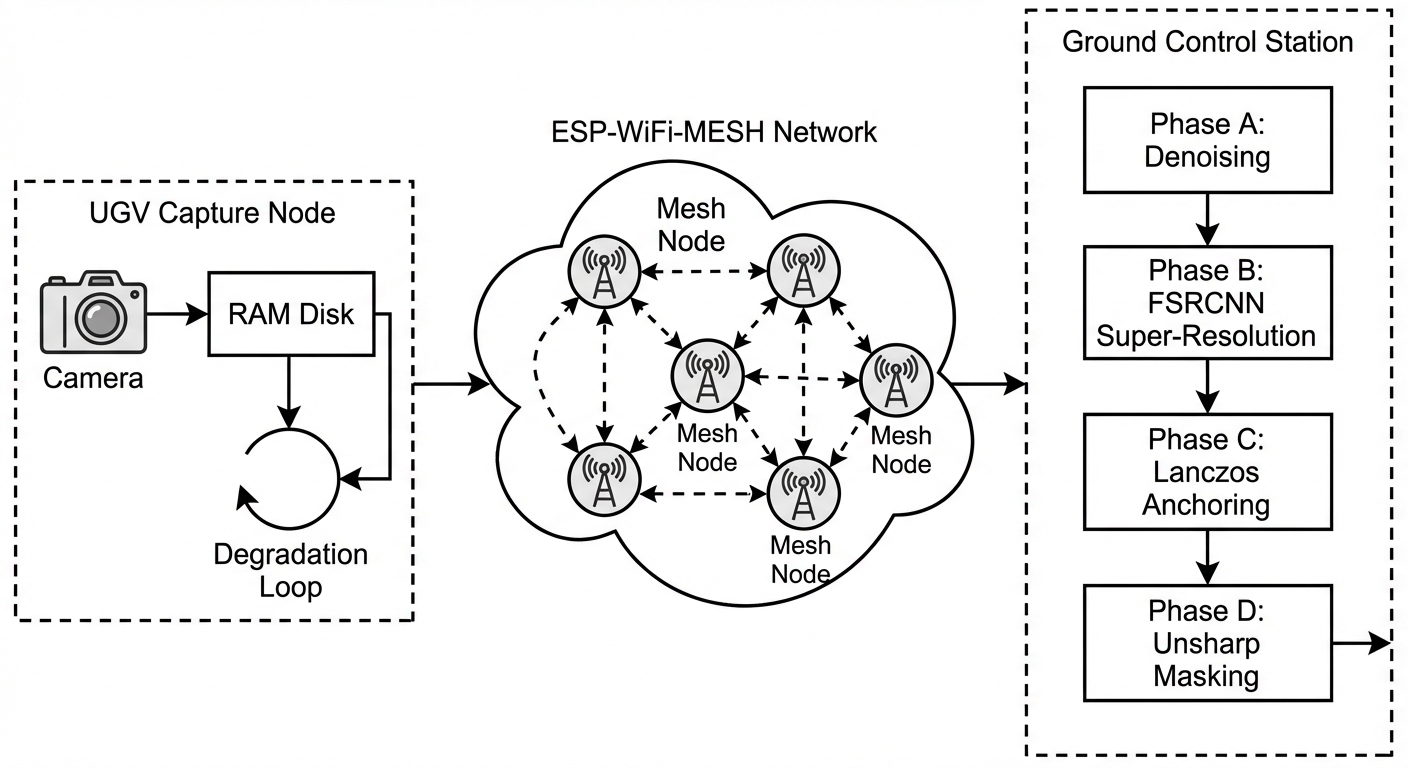
\includegraphics[width=0.95\textwidth]{figures/mesh_methodology.jpeg}
\caption{Mesh network image transmission and AI reconstruction pipeline diagram.}
\label{fig:mesh_methodology}
\end{figure}

\FloatBarrier

\textbf{1. Remote Trigger and Mesh Egress:} The pipeline is initialized manually by a human operator polling a local HTTP endpoint (\texttt{/mesh\_snap}). A background thread immediately acquires a mutual exclusion lock to prevent overlapping requests, flushes the UART buffer, and initiates a high-precision timer to calculate the exact Round Trip Time (RTT). The command payload (\texttt{[ROOT] /snap}) is transmitted at 115200 baud to the local ESP32 root node, which orchestrates the command upstream across the ESP-WiFi-MESH network to the target Raspberry Pi.

\textbf{2. Asynchronous Live Capture and Hardware Preservation:} To preserve the hardware, the target Raspberry Pi avoids invoking a new camera capture instance, which is slow and resource-intensive. Instead, a continuous GStreamer pipeline pulls 640$\times$480 video at 25 FPS from the local camera. Using a \texttt{tee} element, one branch multiplexes H.264 video to a UDP sink for normal high-bandwidth streaming. The secondary branch exists purely for mesh snapshots: it writes raw decoded frames via a \texttt{multifilesink} directly to a volatile \texttt{tmpfs} RAM disk (\texttt{/dev/shm/latest\_frame.jpg}). By over-writing a single file entirely in RAM, this zero-wear memory logging bypasses the physical SD card, preventing flash memory burnout while providing immediate frame access for the degradation script.

\textbf{3. Node-Side Degradation and Compression Logic:} Upon receiving the \texttt{[SNAP]} command over UART, the Pi invokes a suppression loop. The latest frame is loaded from RAM and converted to RGB. To ensure mesh stability, a hard ceiling of 8192 bytes (8\,kB) is strictly enforced. An iterative envelope-shrinking algorithm starts at a 320$\times$240 resolution with WebP compression at 60\% quality (WebP was chosen as it yields historically $\sim$30\% smaller byte footprints compared to JPEG for structurally identical content). If the memory buffer exceeds 8\,kB, the script destructively decreases the resolution by 20\% and the WebP quality by 15. This loop repeats dynamically until the image fits the 8\,kB limit. Finally, because mesh protocols handle binary data poorly, the binary WebP buffer is encoded into Base64 (increasing file size by exactly 33\%), suffixed with a \texttt{[SNAP]} header, and flushed down the UART port to route back home.

\textbf{4. Mesh Transport and Receiver Ingestion:} The massive data chunk traverses the mesh protocols back downstream. The operator-side HTTP server holds the connection open with a loop bound to a strict 15.0-second timeout. It rapidly polls the serial interface, forcing the receiving thread to wait until it securely buffers the entire fragmented transmission (sometimes >4,000 ASCII characters) before returning line data. The Base64 string is validated, sliced of its header, and decoded natively back into a pure binary WebP stream.

\textbf{5. Advanced AI Operator-Side Reconstruction Phase:} Because a severely degraded 8\,kB WebP image (e.g., 256$\times$192, highly compressed) is notoriously difficult to discern visual context from, a four-phase computer vision pipeline hallucinates lost details to make it readable for human supervisors. First, the binary stream is decoded into a standard color matrix. 
\begin{itemize}
    \item \textbf{Phase A: Denoising.} Heavy WebP compression induces structural ``pixel blocks'' that look geometric. To prevent the AI from incorrectly sharpening these blocks, the image is vigorously scrubbed using a non-local means denoising algorithm, washing away the compression grid while preserving natural edge slopes.
    \item \textbf{Phase B: AI Super Resolution.} A pre-trained Fast Super-Resolution Convolutional Neural Network (FSRCNN) \cite{dong2016fsrcnn} model mathematically hallucinates high-frequency details from the washed matrix. It recognizes underlying physical geometries and scales the internal resolution exactly $2\times$ larger.
    \item \textbf{Phase C: Lanczos Spatial Anchoring.} The image is passed through a simple resize to an anchored 640$\times$480 dimension using a Lanczos resampling filter, mitigating mathematically sharp alias edges from the unpredictable aspect ratio changes induced during the Pi's active compression loop.
    \item \textbf{Phase D: Aggressive Unsharp Masking.} To counteract the soft ``painterly'' focus introduced by the neural network upscale, a heavy Gaussian blur is overlaid and mathematically subtracted. This weighted subtraction forces an aggressive clarity curve so geometric edges ``pop'' to the human eye.
\end{itemize}

\textbf{6. Egress and Benchmark Telemetry:} Finally, the finished AI-corrected matrix is packed back into a visually lossless WebP envelope and delivered via a standard HTTP \texttt{200 OK} response to the operator's browser. The script calculates the exact Round Trip Time, running mathematics to verify Base64 mesh size, hardware CPU AI upscale time, true image size, and effective throughput (kB/s) for real-time mesh diagnostic logging.


\section{User Interface}

\subsection{UI Component 1: Operator Dashboard}

The ground control station provides a web-based operator dashboard that serves as the primary human--machine interface for mission supervision and manual override. The dashboard is a JavaScript frontend that communicates with the FastAPI \cite{fastapi} perception backend and with the robot via rosbridge \cite{rosbridge} over WebSocket. It runs in a standard browser and requires no additional client software.

The dashboard displays multiple camera streams: the main USB webcam feed, the rear ESP32-CAM feed, and when available a depth or costmap view. The live occupancy map is rendered with the current robot pose and hazard markers (spheres and labels at SLAM coordinates, colour-coded by severity) that are updated from the AI perception pipeline. A detections panel shows the list of identified objects (fire/smoke, extinguisher, human) with severity badges and timestamps. The operator can trigger frame processing by capturing a snapshot from the main camera; the result (YOLO detections, LLM scene and hazard output, and spatial decision) is displayed and the map annotations update accordingly. Natural-language summaries from the LLM provide a mission narrative for situational awareness.

Teleop controls allow the operator to override autonomy at any time: velocity commands can be sent via a virtual joystick or keyboard, and the robot responds to manual input while the exploration stack can resume when manual control is released. Battery level, network status (across Wi-Fi, 4G, mesh, and LoRa), and SLAM pose are shown so that the operator can assess system health and connectivity. The interface is designed for use on laptops or tablets in the field. High-level mission controls (e.g.\ start exploration, pause, return to base, emergency stop) can be integrated where supported by the underlying ROS~2 services and actions.

% --- FIGURE: GCS dashboard ---
\begin{figure}[htbp]
\centering
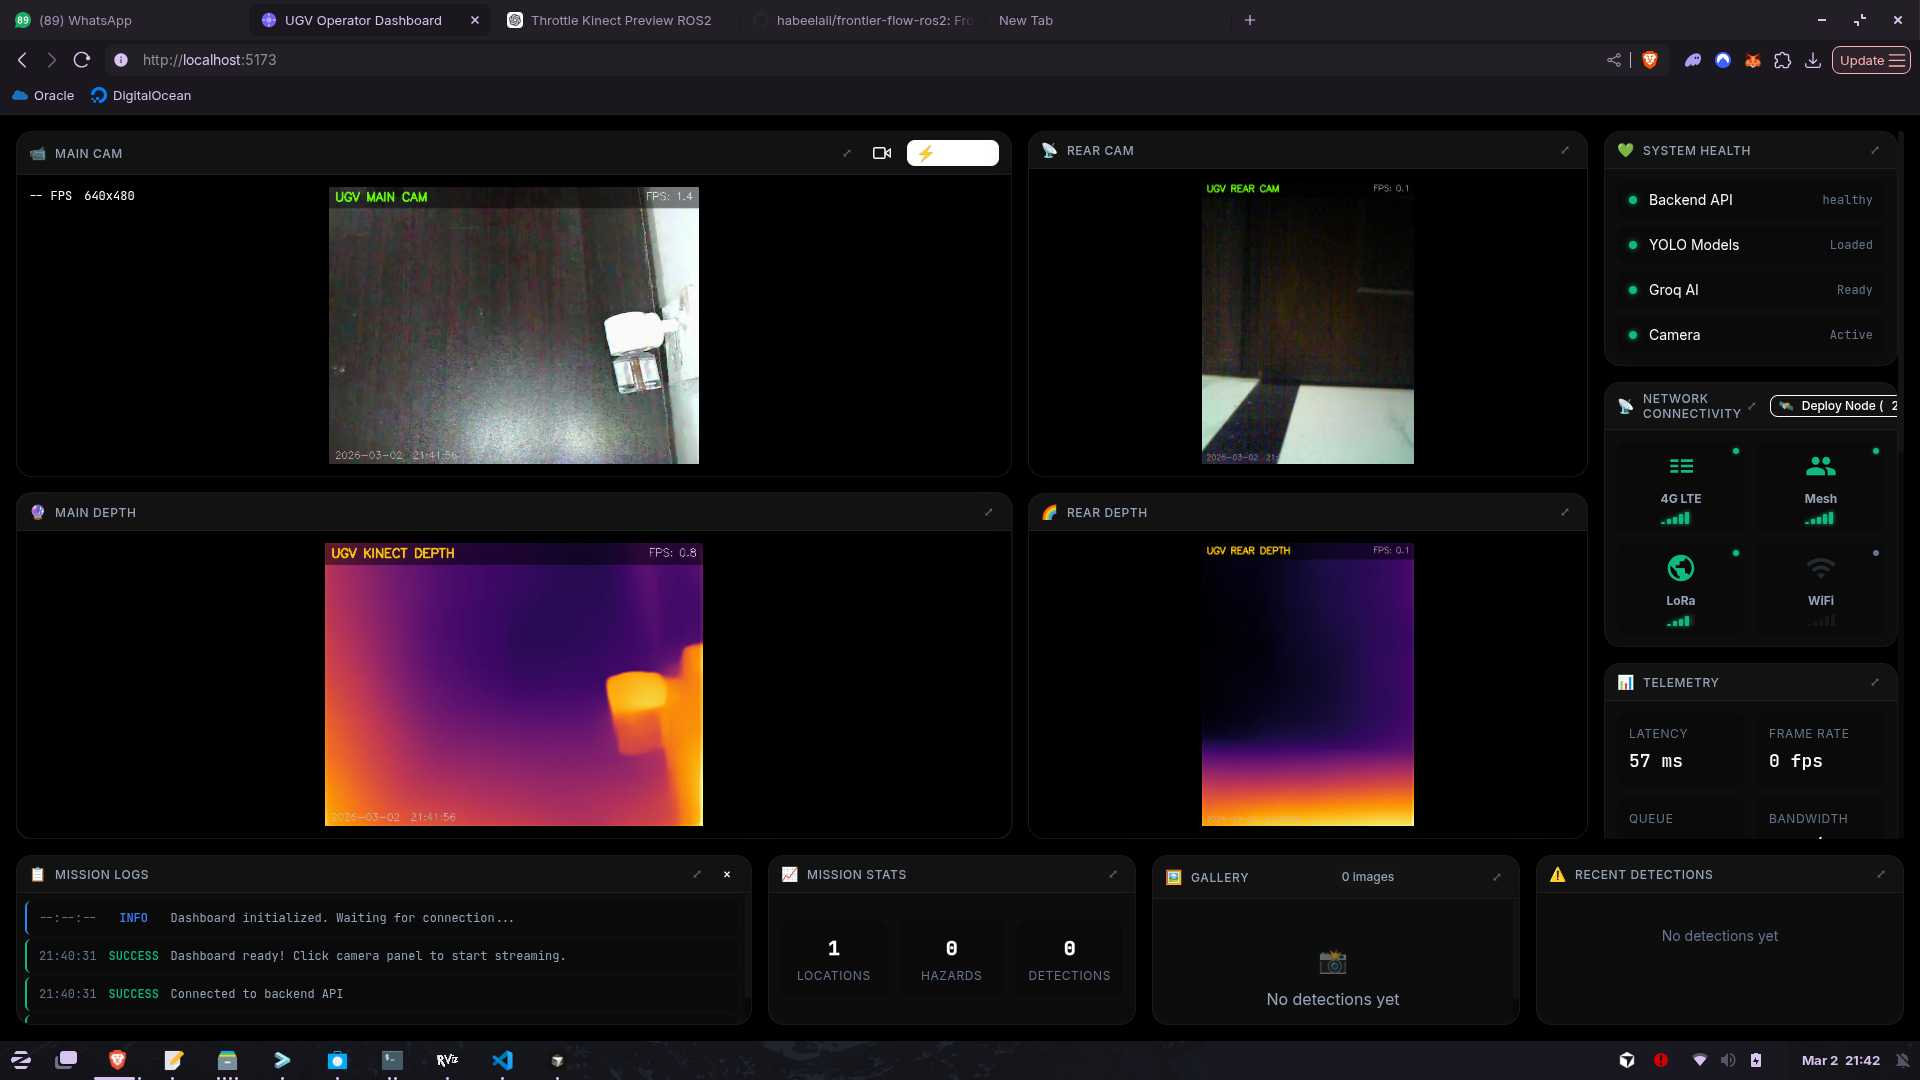
\includegraphics[width=0.9\textwidth]{figures/dashboard.png}
\caption{GCS operator dashboard: camera streams, map, detections, teleop, battery/network.}
\label{fig:dashboard}
\end{figure}

\section{Evaluation}

The implemented system was evaluated in a real indoor test environment to assess mapping and localization, communication performance, detection and AI perception, and the impact of AI map prediction on frontier-based exploration. The test space was a university department floor approximately 40\,m deep and 30\,m wide, with a long corridor between lobbies and rooms on both sides, representative of office or institutional buildings where search-and-rescue or damage assessment might be conducted. The operator was stationed outside the department to simulate a remote command post.

Evaluation covered: (1) \textbf{Mapping and localization} --- real-time Cartographer performance on the Pi~4, loop closure behaviour, drift in feature-rich vs.\ feature-poor regions, map resolution and consistency over full runs; (2) \textbf{Communication} --- throughput and range for Wi-Fi (line-of-sight and through rooms), 4G hotspot, ESP-WiFi-MESH with up to two deployable nodes, and LoRa indoors; (3) \textbf{Detection and AI} --- YOLOv8 mean average precision on disaster-relevant imagery, per-frame inference time on the GCS GPU, end-to-end latency from capture to displayed result over Wi-Fi and over mesh, and LLM scene analysis latency; (4) \textbf{Frontier scoring} --- comparison of exploration with and without the ProxMaP-based map predictor (time to full coverage, area covered at a fixed time, number of frontier goals reached per run). Multiple runs were conducted for each major capability. Communication throughput and range depend on building layout and antenna placement; the values reported were measured in the test environment. The detailed results are reported in Chapter~\ref{ch:results}.

% --- FIGURE: Test environment floor plan ---
\begin{figure}[htbp]
\centering
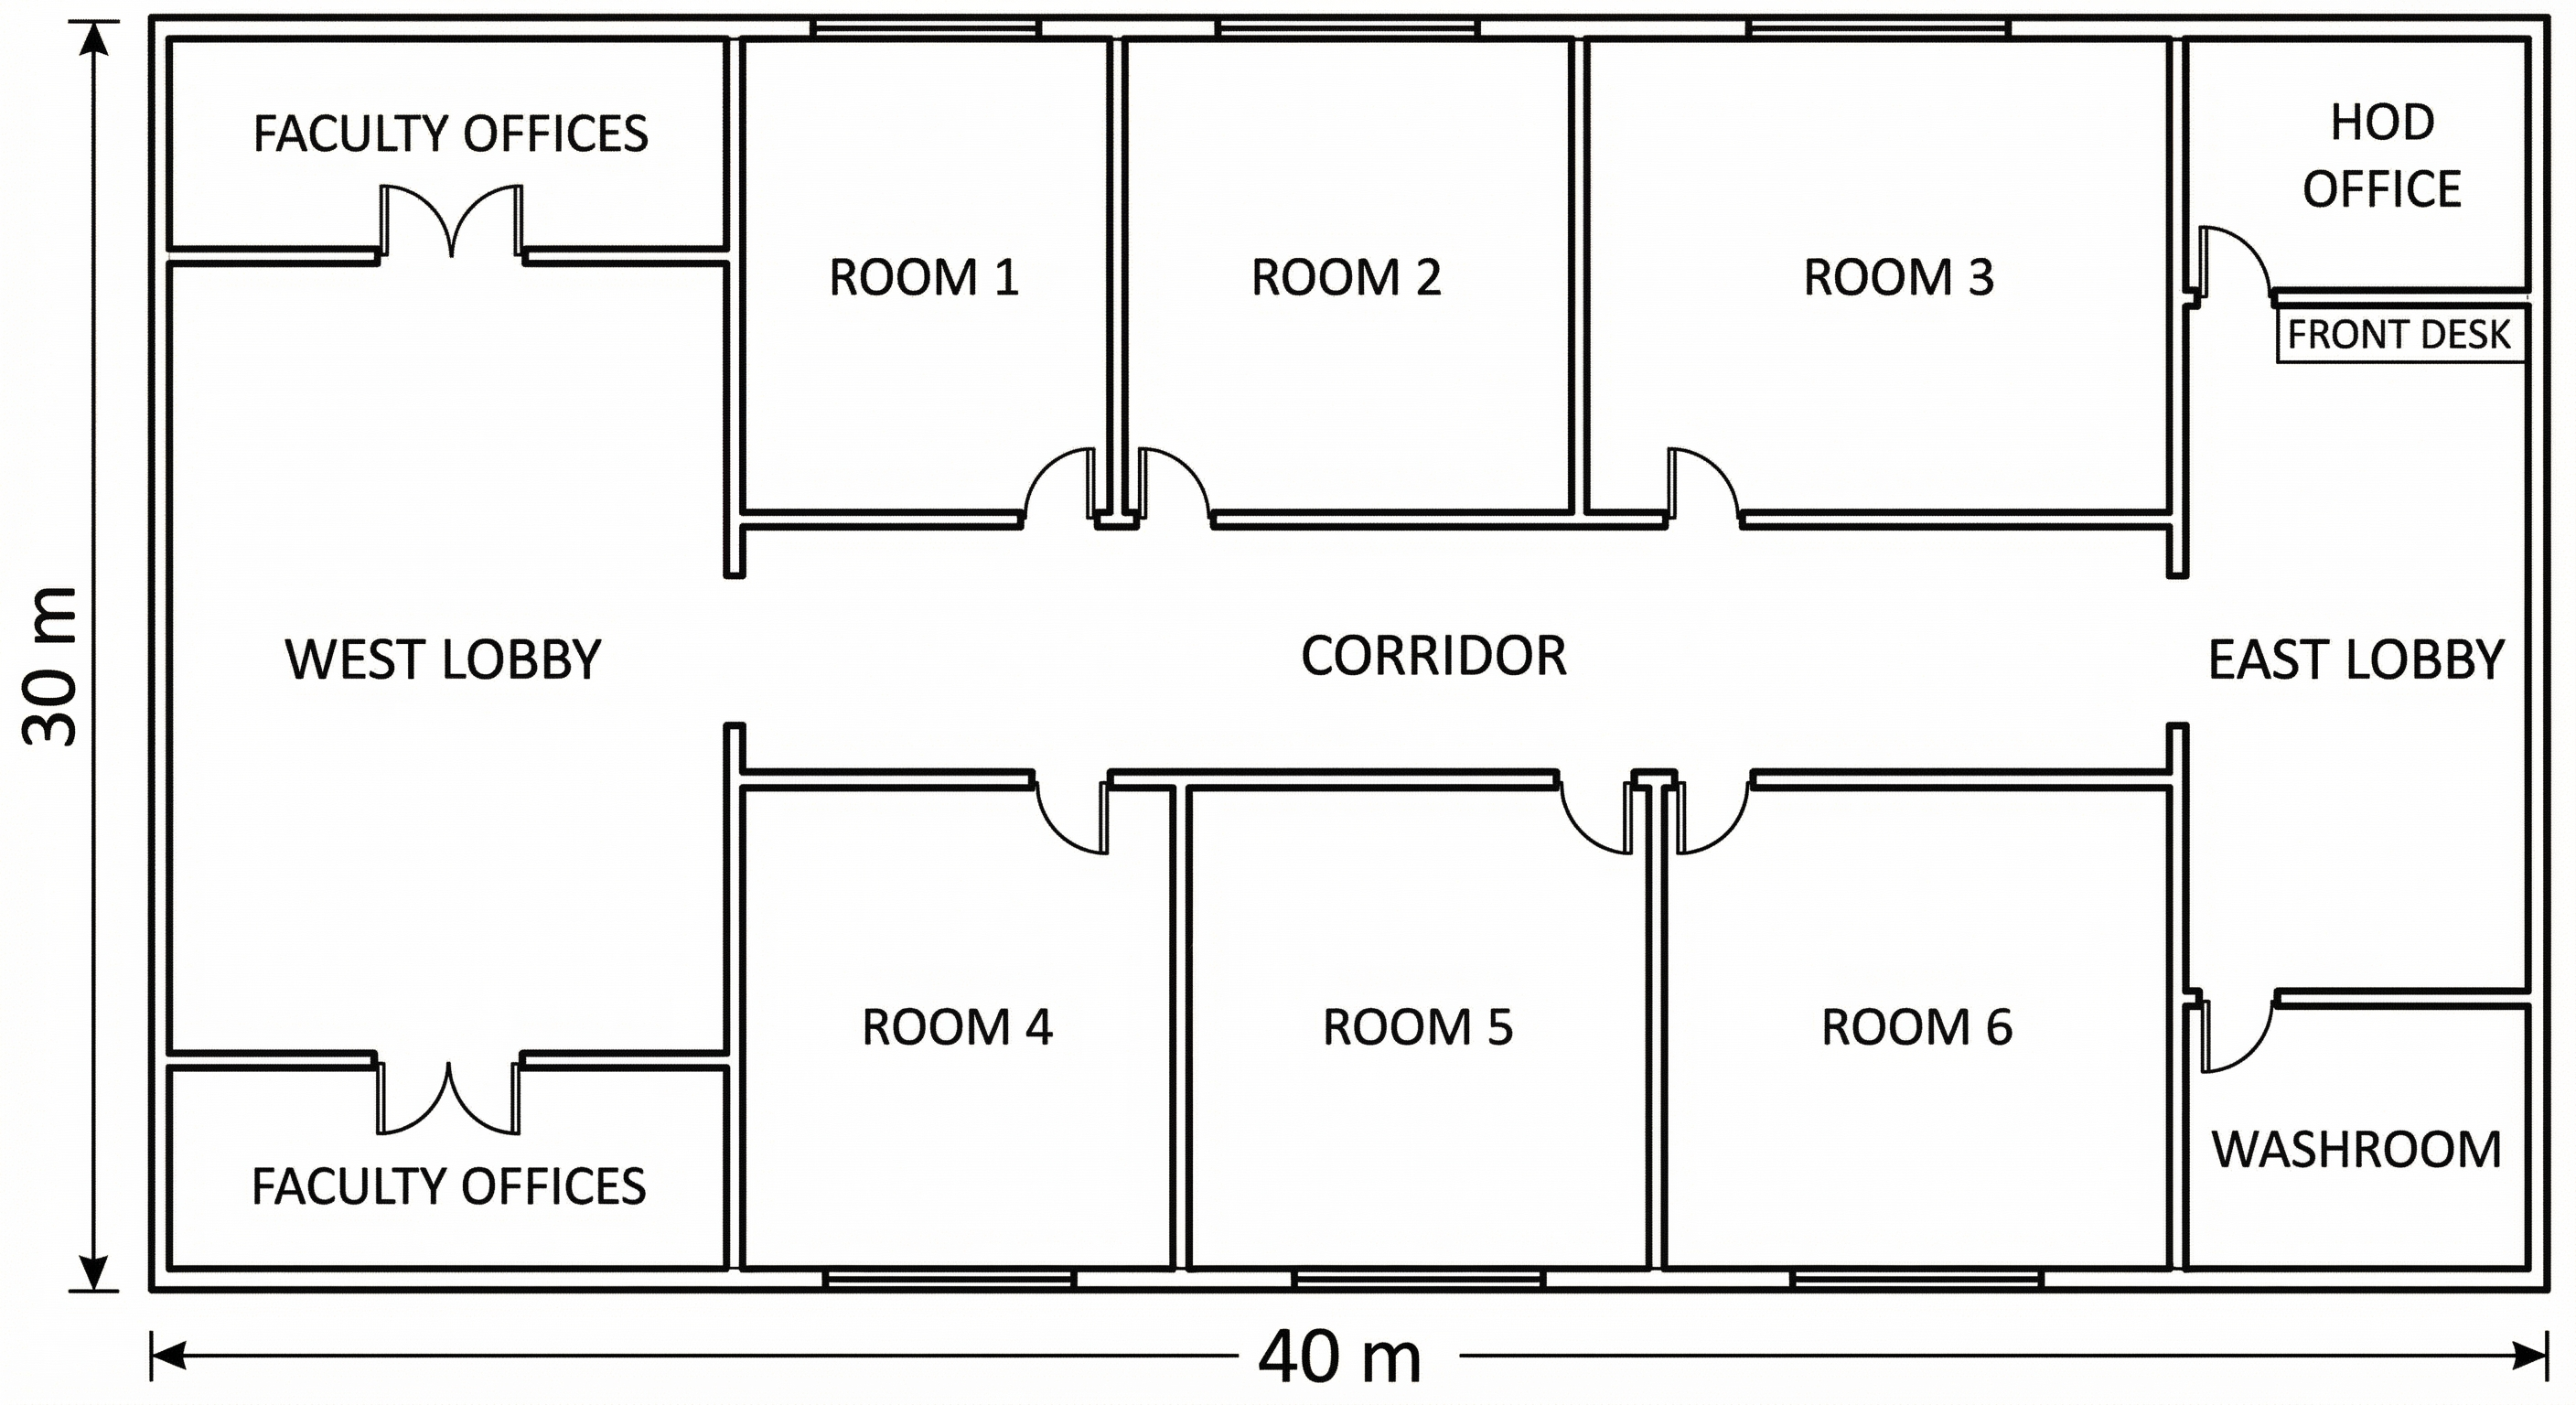
\includegraphics[width=0.75\textwidth]{figures/floor_plan.jpeg}
\caption{Test environment floor plan (approx.\ 40×30\,m).}
\label{fig:floorplan}
\end{figure}

\section{Unit Testing}

Unit-level testing was applied to individual software and hardware components before and during integration.

\textbf{SLAM and navigation.} Cartographer \cite{hess2016} was tested with live LiDAR data and with recorded bag files to verify real-time pose updates, submap generation, and loop closure. The map-to-odom and base\_link-to-laser\_frame transform chain was validated. Nav2 \cite{nav2dwb} global and local planners were exercised in isolation with sample occupancy grids to confirm path generation and costmap behaviour; the Kinect v1 point cloud was verified to appear correctly in the local costmap layer.

\textbf{Frontier explorer and map predictor.} The custom frontier explorer was tested for frontier cell detection (including the 5×5 window for Cartographer's border), 8-connected BFS clustering, and scoring with and without the predicted map. The map predictor node (ProxMaP-style U-Net \cite{sharma2022}) was tested on 128×128 map crops to ensure correct input formatting and output (predicted free/occupied/unknown) and that the predicted map topic was published at the expected rate.

\textbf{Perception pipeline.} YOLOv8 \cite{yolov8} models (fire/smoke, extinguisher, human) were run on sample images to verify detection output and merging. The FastAPI \cite{fastapi} endpoint for frame processing was tested with synthetic or captured images and SLAM coordinates to confirm structured JSON output (scene description, hazard, persons\_seen, needs\_annotation). X-SDM and person profiling logic were checked for revisit vs.\ new-location classification and for correct annotation publishing to the ROS~2 topic.

\textbf{Communication.} ESP32 DevKit mesh nodes running ESP-WiFi-MESH \cite{espmesh} were tested for join and self-healing behaviour; deployment and routing-table update were verified when nodes were added. LoRa link was tested for basic telemetry and return-to-base command delivery at indoor ranges. Wi-Fi and 4G connectivity and fallback to mesh (and image-over-mesh) were tested in the target environment.

Unit tests were documented with pass/fail and observed outcomes; where components depended on ROS~2 or hardware, tests were run in the integration environment or in simulation where applicable. Figure~\ref{fig:gazebo} shows the simulation environment used where applicable.

\begin{figure}[htbp]
\centering
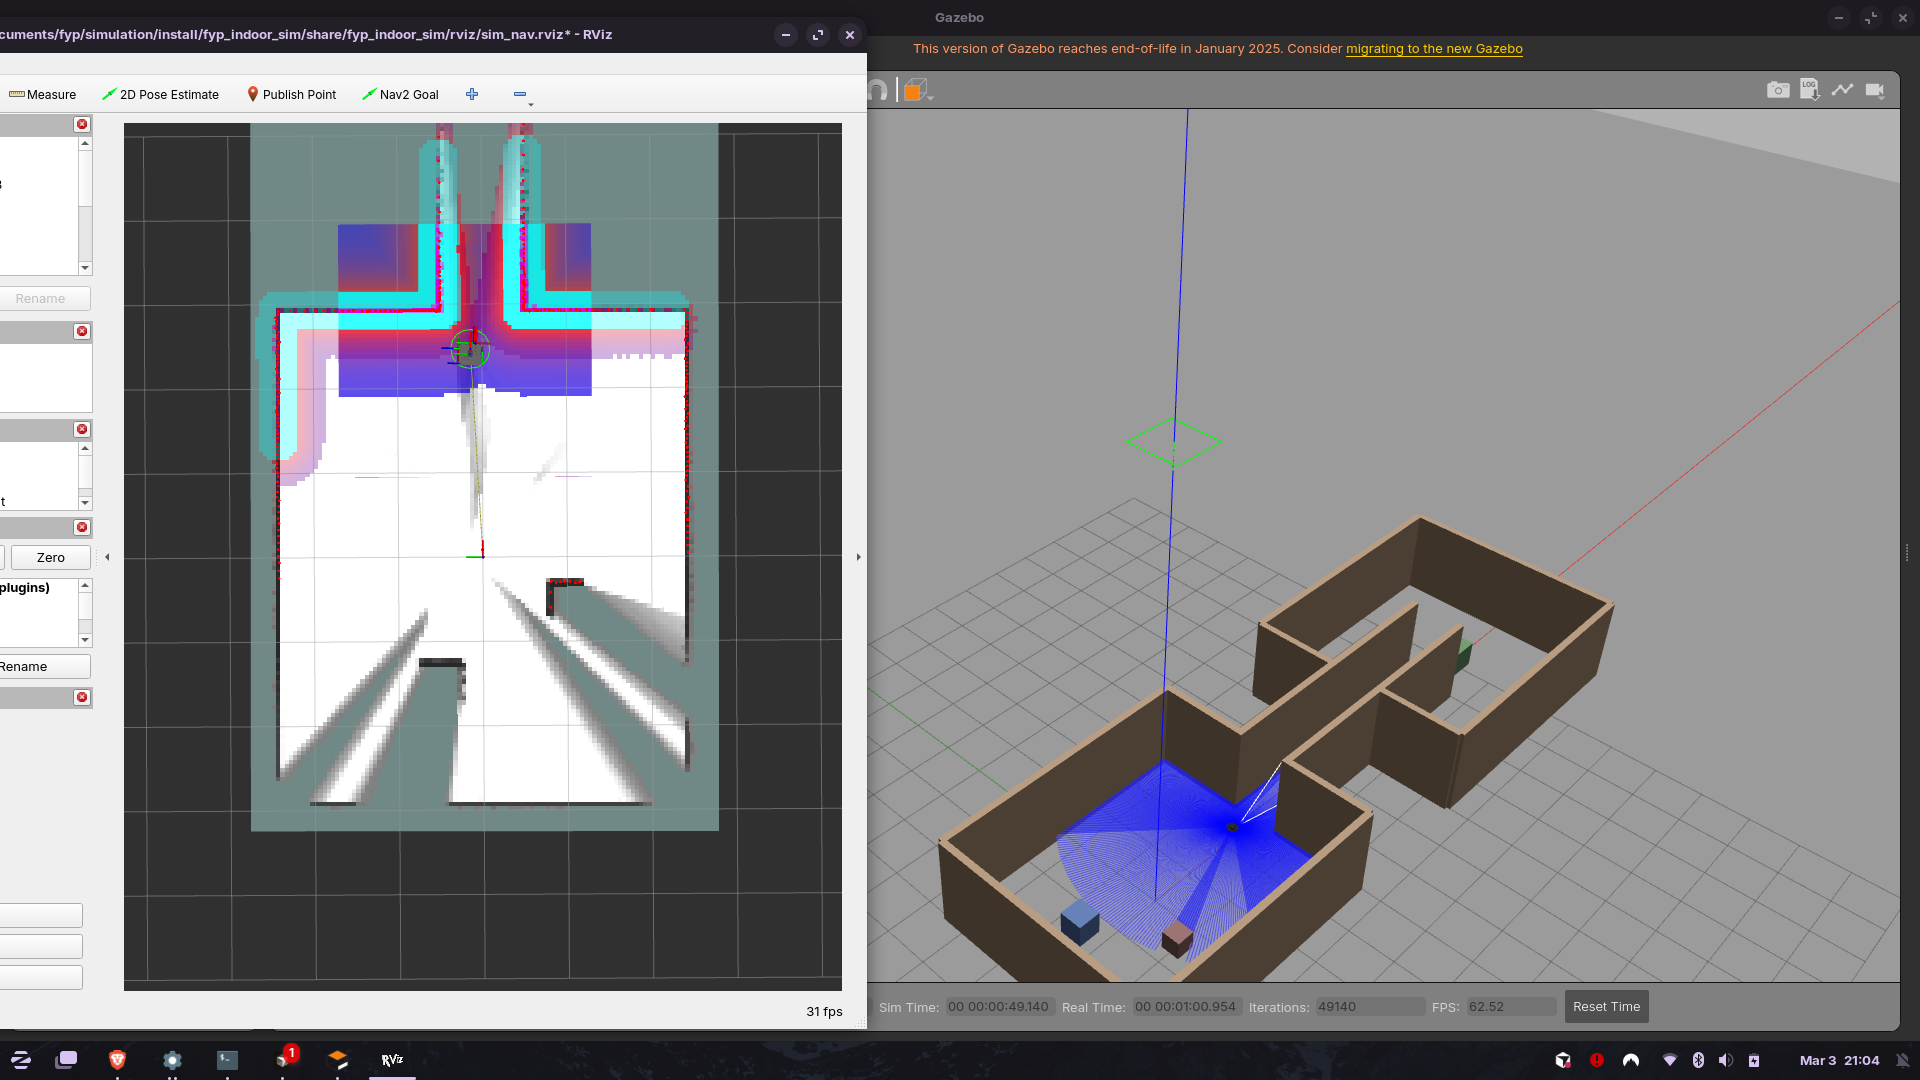
\includegraphics[width=0.8\textwidth]{figures/gazebo.png}
\caption{Simulation environment (Gazebo).}
\label{fig:gazebo}
\end{figure}

\section{Function Testing}

\subsection{Testing Requirements (by Function)}

Functional testing was designed around three requirement categories aligned with the system's main functions:

\textbf{Requirement A --- Mapping and exploration.} The system shall produce a consistent 2D occupancy map of the test environment using Cartographer with scan-matching and loop closure; loop closure shall reduce cumulative drift when the robot revisits areas. The frontier explorer shall select frontier goals and send them to Nav2; exploration shall complete when no valid frontiers remain or when the operator aborts. The AI map predictor shall be used during exploration to prioritise frontiers that lead to more free space.

\textbf{Requirement B --- Communication.} The system shall maintain at least one usable link among Wi-Fi, 4G, mesh, and LoRa in the test environment. When Wi-Fi or 4G is lost, the system shall fall back to mesh when nodes are deployed; deployed nodes shall be added to the routing table and form a self-healing mesh. When only mesh is available, image transfer shall use dynamic WebP compression (up to 8\,kB) and Base64 encoding, with AI-driven operator-side reconstruction. LoRa shall carry position, battery, and return-to-base commands when other links are unavailable.

\textbf{Requirement C --- Perception and GCS.} Detections (fire/smoke, extinguisher, human) and LLM-generated scene and hazard summaries shall appear on the dashboard. X-SDM shall classify frames as revisit or new location where applicable, and person profiling shall support map annotations for newly seen persons. The operator shall be able to override autonomy via teleop controls and to view camera streams, the live map, detections, and battery/network status.

These requirements were used to design the function test scenarios and pass criteria described below.

\subsection{Testing Requirements (by Scenario) and Execution}

Function tests were executed in the same 40×30\,m indoor test environment used for evaluation. The following scenario-based requirements were applied:

\textbf{Scenario 1 --- Full autonomous run.} The UGV was powered on and the GCS connected via Wi-Fi or 4G. After initialization (3--5 minutes), exploration was started from a consistent initial pose. Pass criteria: the robot built a coherent map, selected and reached frontier goals, and completed or was stopped by the operator without critical failure. Requirement A was verified.

\textbf{Scenario 2 --- Communication fallback and node deployment.} With the UGV in operation, connectivity was varied (e.g.\ operator or UGV moved so that direct Wi-Fi degraded). When two mesh nodes were deployed along the path, the mesh was verified to extend coverage and nodes were confirmed in the routing table. In conditions where only mesh or only LoRa was available, telemetry and return-to-base were verified. Requirement B was verified.

\textbf{Scenario 3 --- Perception and operator interface.} During runs, the operator triggered frame processing and confirmed that detections and LLM summaries appeared on the dashboard, that map markers (hazards, persons) were placed at correct locations, and that teleop override could take control. Battery and network status were monitored. Requirement C was verified.

Test execution followed a short checklist: power-on and link check, sensor and SLAM verification, start exploration, observe mapping and frontier behaviour, exercise comms fallback and node deployment where applicable, and exercise perception and teleop. Results were recorded and used to obtain the quantitative results reported in Chapter~\ref{ch:results}.
